\documentclass[../sdrg,../../main.tex]{subfiles}
\begin{document}
\section{Fixed Points and the Random Singlet Phase}

If we look for fixed point solutions for the RG flow (3.10), a natural approach is to rescale $\zeta$ to an appropriate power of $\Gamma$, $\kappa$, since in this model the randomness always leads to a critical point.\\

By defining
\begin{equation}
    \eta = \frac{\zeta}{\Gamma^\kappa}
\end{equation}
the distribution transforms to
\begin{equation}
    P(\zeta,\Gamma)=\frac{1}{\Gamma^\kappa}Q(\eta,\Gamma)
\end{equation}
and therefore the flow equation becomes
\begin{equation}
    \Gamma\pdv{Q}{\Gamma}=\kappa\left( Q+\eta\pdv{Q}{\eta}\right)+\Gamma^{1-\kappa}\left(\pdv{Q}{\eta}+Q(0,\Gamma)\int_{0}^{\eta}\dd\eta'Q(\eta',\Gamma)Q(\eta-\eta',\Gamma)\right)
\end{equation}

For $\kappa>1$ the second term vanishes, leaving the fixed point equation as
\begin{equation}
    \pdv{Q}{\eta}=-\frac{Q}{\eta}
\end{equation}
giving the trivial solution of $Q(\eta)=\flatfrac{C}{\eta}$, which diverges for small $\eta$, i.e. approaching the strongest bond. \\

For $\kappa<1$ the second term dominates, leaving tthe fixed point equation as
\begin{equation}
    \pdv{Q}{\eta}=-Q(0)\int_{0}^{\eta}\dd\eta'Q(\eta')Q(\eta-\eta')
\end{equation}
who's solution, using Laplace transformations, can be shown to oscillate in sign for big $\eta$. \cite{fernandez}.\\

Both the aforementioned solutions are unphysical when it comes to the behaviour of fixed points, thus the only physical solution left is $\kappa = 1$ as a possible scale exponent, leaving us only with
\begin{equation}
    \Gamma\pdv{Q}{\Gamma}= Q(\eta,\Gamma) + (1+\eta)\pdv{Q}{\eta}+Q(0,\Gamma)\int_{0}^{\eta}\dd \eta'Q(\eta',\Gamma)Q(\eta-\eta',\Gamma)
\end{equation}

Looking for solutions of $Q^{*}(\eta)$, independent of $\Gamma$, and therefore $\pdv{Q}{\Gamma}=0$, we get the fixed point equation, which has a one-parameter family of solutions, parametrized by $Q_{0}^{*}=Q^{*}(0)$.\\

By Laplace transforming $Q\rightarrow \hat{Q}$,
\begin{equation}
    z\pdv{\hat{Q}}{z}=z\hat{Q}+Q_{0}[\hat{Q}^{2}-1]
\end{equation}
where $Q_{0}$ is constrained by
\begin{equation}
    Q_{0}=Q(0)=\lim_{\eta\rightarrow0^{+}} \frac{i}{2\pi i}\int_{c-i\infty}^{c+i\infty}\dd z\ \hat{Q}(z)e^{z\eta}
\end{equation}
and by linearizing $\hat{Q}$ via the transformation
\begin{equation}
    \hat{Q}=\frac{-z}{uQ_{0}}\dv{u}{z}
\end{equation}
equation (3.15) becomes
\begin{equation}
    \dv[2]{u}{z}+\left(\frac{1}{z}-1\right)\dv{u}{z}-\frac{Q_0^2}{z^2}u=0
\end{equation}
Using the Frobenius method\cite{fernandez} we find that $Q_{0}=Q(0)$ parametrizes a family of solutions to the above equation, which when plugged into (3.14) gives the Laplace transformation of the distribution. Using the inverse Laplace transform is then the fixed points we were looking for.\\

To narrow down the possible fixed point solutions, we must distinguish between whether or not $Q_{0}$ is an integer. If $2Q_{0}$ is not an integer, instead of using the Frobenius method, we can use the simpler
\begin{equation}
    u = \sum_{n=0}^{\infty}u_nz^{n}
\end{equation}
where $u_{n}$ is given by the recursion relation
\begin{equation}
    u_{n+1}=\frac{n-Q_{0}}{(n+1)(n+1-2Q_{0})}u_{n}
\end{equation}
implying that for large positive z, $u(z)\sim z^{a}e^{z}$ so that $\hat{Q}\approx-\flatfrac{z}{Q_{0}}$ which is unphysical\cite{fisher}. Therefore $2Q_{0}=m$ is an integer, which implies a $z^{m}\ln{z}$ part in $u$\cite{fisher} forcing a $\flatfrac{1}{\eta^{2Q_{0}+1}}$ tail in $Q(\eta)$. The only exception is if $m=2$, meaning $Q(0)=1$, where in this case $u=1+z$.\\

In the case where $Q_{0}=1$, the general form of $\hat{Q}$ is explicitly given by
\begin{equation}
    \hat{Q}=\frac{1+C'e^z(1-z)}{1+z+C'e^z}
\end{equation}
where the only value of $C'$ that gives the proper large $z$ behaviour $\hat{Q}\approx\flatfrac{Q_{0}}{z}$, corresponding to the discontinuity at $\eta=0$ is $C'=0$.\\

This means that the only fixed point that behaves well is
\begin{equation}
    \hat{Q}=\frac{1}{1+z}
\end{equation}
yielding
\begin{equation}
    Q^{*}(\eta)=e^{-\eta}\Theta(\eta)
    \label{eq:rss}
\end{equation}
where $\Theta(\eta)$ is the Heaviside step function. This is the random singlet fixed point distribution, which can be shown to be stable under pertubations exponentially decaying in $\eta$.\cite{fisher}\\

If we want to express this distribution in terms of the original spin chain distribution, remembering that $\kappa = 1 $
\begin{equation}
    P^{*}(\zeta,\Gamma)=\frac{1}{\Gamma}e^{\sfrac{-\zeta}{\Gamma}}\Theta(\zeta)
\end{equation}
and by reverting back from the logarithmic parameters to our original bonds,
\begin{equation}
    P^{*}(J,
    \Omega) =\frac{\alpha}{\Omega}\left(\frac{\Omega}{J}\right)^{1-\alpha}\Theta(\Omega-J)
\end{equation}
where
\begin{equation}
    \alpha = \flatfrac{1}{\Gamma}=-\flatfrac{1}{\ln \Omega}
\end{equation}


If we remember the RG process, during each step we paired the two spins with strongest bond in a singlet, replacing them with an effective bond between the neighbouring spins. Repeating this process enough times, the total effective bond between two spins at along distance can become the strongest bond in the chain, causing the two spins to be paired in a long ranged singlet.\\

\begin{figure}[h!]
    \centering
    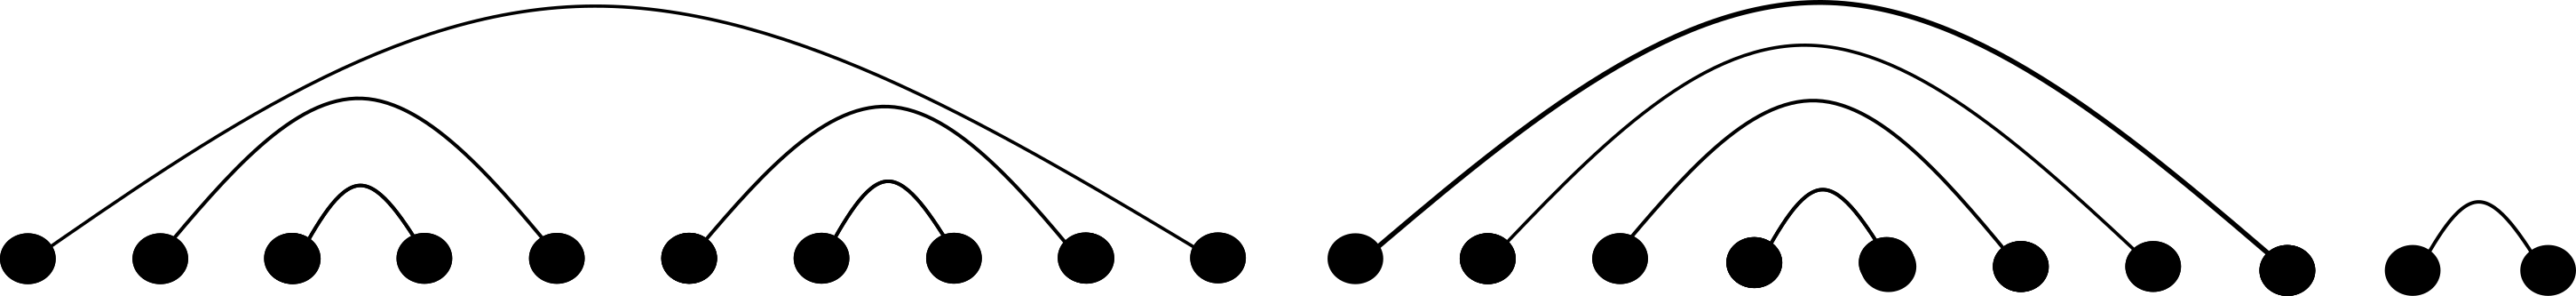
\includegraphics[scale = 0.15]{Chapter4/Figures/RSP.png}
    \caption{A schematic of the random singlet phase. Pairs of spins, connected via bonds form singlets over arbitrarily long distances. Notice that bonds do not overlap.}
\end{figure}

At low energies, the system consists mostly of pairs of spins coupled together into singlets over arbitrarily long distances, shown in Figure 3.1. This critical point, described by the distribution (3.23) is known as the random singlet phase.
\end{document}